
\section{Dominio cerrado (Popescu/World)}
\subsection{Introducción}
\begin{frame}
\frametitle{Introducción}
\begin{itemize}
  \item Sistema que implementa el modelo propuesto por Popescu en [Popescu et al. 2003a] y  [Popescu et al. 2003b].
  \item Define concepto de tratabilidad semántica y traduce preguntas semánticamente tratables en consultas SQL
  \item Código implementado en java, accesible en http://github.com/julian3833/popescu-world
  \item Testeado sobre base de datos relacional de juguete provista por MySQL, llamada World, con información geográfica básica de países, ciudades e idiomas.
  \item Sistema de funcionalidad acotada con soporte solo para el inglés.
\end{itemize}
\end{frame}

\subsection{Modelo teórico}

\begin{frame}
  \frametitle{Dominio de problemas}
   \begin{block}{Dominio acotado y específico}<1->
      \begin{itemize}
          \item Restaurants, bancos, vuelos, libros, etcétera (pero solo uno)
          \item Bases de datos relacionales $\rightarrow$ datos estructurados
          \item Question answering como interfaz para una base de datos
          \item Traducir pregunta a SQL
      \end{itemize}
    \end{block}
\end{frame}

\begin{frame}
  \frametitle{Ejemplo}
  \begin{block}{Pregunta}<2->
      When did Albert Einstein die?
  \end{block}
  \begin{columns}<3->
      \begin{column}{.5\textwidth}
      \end{column}
      \begin{column}{.1\textwidth}
      \begin{tikzpicture}[>=stealth, rotate border/.style={shape border uses incircle, shape border rotate=270}]
              \node[rotate border=-40, fill=black, minimum height=1.0cm, single arrow, single arrow head extend=.3cm, single arrow head indent=.1cm, inner sep=1.5pt] (arrow) {};
          \end{tikzpicture}
      \end{column}
      \begin{column}{.3\textwidth}
          %Question Answering
      \end{column}
      \begin{column}{.5\textwidth}

      \end{column}
  \end{columns}

  \begin{exampleblock}{Consulta SQL}<3->
      \textbf{SELECT} death\_date \textbf{FROM} scientists

      \textbf{WHERE} name $=$ `Albert Einstein'
  \end{exampleblock}
  \begin{columns}<4->
      \begin{column}{.5\textwidth}
      \end{column}
      \begin{column}{.1\textwidth}
      \begin{tikzpicture}[>=stealth, rotate border/.style={shape border uses incircle, shape border rotate=270}]
              \node[rotate border=-40, fill=black, minimum height=1.0cm, single arrow, single arrow head extend=.3cm, single arrow head indent=.1cm, inner sep=1.5pt] (arrow) {};
          \end{tikzpicture}
      \end{column}
      \begin{column}{.3\textwidth}
          %Question Answering
      \end{column}
      \begin{column}{.5\textwidth}

      \end{column}
  \end{columns}

  \begin{alertblock}{Respuesta}<4->
      April 18th, 1955
  \end{alertblock}

\end{frame}


\begin{frame}
  \frametitle{Modelo teórico}
      \begin{itemize}
          \item Popescu et al. $\rightarrow$ QADB, Precise
          \item Tratabilidad semántica de una pregunta $q$ en el contexto de una DB $d$.
          \item Las preguntas no tratables se rechazan, las tratables se traducen.
          \item Motivación: no se puede fallar activamente (mal interpretar)
      \end{itemize}
\end{frame}





\begin{frame}
  \frametitle{Tratabilidad semántica / motivación}
      \begin{itemize}
          \item La complejidad de las preguntas en lenguaje natural es arbitrariamente grande.
          \item Las preguntas semánticamente tratables son preguntas fáciles pero abarcativas
          \item Distinguir un subconjunto 1) \textit{tratable} y 2) \textit{abarcador}
          \item Rechazar y pedir reformulación de las no tratables
          \begin{itemize}
            \item Es mejor no dar respuesta a dar una mala. Conservar la confianza en el sistema.
          \end{itemize}
      \end{itemize}
\end{frame}

\begin{frame}
  \frametitle{Tratabilidad semántica / idea coloquial}
    \begin{block}{Tratabilidad semántica en el contexto de una DB}<1->
      \begin{itemize}
          \item Una Q-word (Qué, quién, cuándo, dónde, etc.)
          \item Pares de atributos y valores
          \item Valores sueltos
          \item Términos no significativos y menciones a relaciones
          \item Por ejemplo:
            \begin{itemize}
              \item ¿{\color{green}Qué} {\color{orange}bancos} de la {\color{red}empresa Credicoop} están localizados en el {\color{blue}barrio} de {\color{blue}Coghlan}?
              \item ¿{\color{green}Quién} era el {\color{red}presidente} de {\color{red}México} en {\color{orange}1993}?
            \end{itemize}
      \end{itemize}
    \end{block}
\end{frame}

\fontsize{9.5pt}{7.2}\selectfont
\begin{frame}
  \frametitle{Definiciones (1): Elemento, qword, compatibilidad, token, marcador sintáctico}
   \begin{itemize}
      \item Elementos de una DB: Relaciones, Atributos y Valores
      \item Qwords - pronombres interrogativos
      \begin{itemize}
          \item \{What, where, which, when, who\}
          \item \{Qué, dónde, cuál, cuándo, quién\}
      \end{itemize}
      \item Compatibilidad 
      \begin{itemize}
          \item Valor con sus atributo
          \item Atributos con sus relaciones
          \item Valor con las relaciones de sus atributos
          \item Q-words compatibles con atributoes
          \begin{itemize}
            \item Definición a mano especifica por DB
          \end{itemize}
      \end{itemize}
      \item Token: un conjunto de lemas de palabras de la pregunta que corresponden a un elemento de la base de datos.
      \begin{itemize}
            \item Por ejemplo, \{experiencia, requerir\} y \{experiencia, necesario\} son dos tokens para ``Experiencia Requerida''
      \end{itemize}
      \item Marcador sintáctico: palabras que no aportan a la interpretación de la pregunta, definidas a mano
    \end{itemize}
\end{frame}

\fontsize{9.5pt}{7.2}\selectfont
\begin{frame}
  \frametitle{Definiciones (2): Correspondencia entre tokens y elementos}
  \begin{itemize}
    \item Cada elemento de la base de datos se separa en palabras individuales:
    \begin{itemize}\fontsize{9.5pt}{7.2}\selectfont
      \item “Experiencia Requerida” $\rightarrow$ \{Experiencia, Requerida\}
    \end{itemize}
    \item Se genera un conjunto de sinónimos para cada palabra usando Wordnet:
    \begin{itemize}\fontsize{9.5pt}{7.2}\selectfont
      \item experiencia $\rightarrow$ \{experiencia, conocimiento, habilidad,...\}
      \item requerida $\rightarrow$ \{requerida, necesaria, indispensable,...\}
    \end{itemize}
    \item Se toman los lemas o raíces de todas las palabras
      \begin{itemize}\fontsize{9.5pt}{7.2}\selectfont
        \item experiencia $\rightarrow$ \{experiencia, conocimiento, habilidad,...\}
        \item requerida $\rightarrow$ \{requerir, necesario, indispensable,...\}
    \end{itemize}
    \item Se generan tokens combinando los lemas de los sinónimos de cada elemento:
    \begin{itemize}\fontsize{9.5pt}{7.2}\selectfont
        \item tokens = \{(experiencia, requerir), (conocimiento, requerir), (habilidad, requerir),(experiencia, necesario), (conocimiento, necesario), (habilidad, necesario),(experiencia, indispensable), (conocimiento, indispensable), (habilidad, indispensable)\}
    \end{itemize}
    \item Este conjunto de tokens son los tokens que se corresponden con el elemento
    \item Un token tiene tipos dependiendo a qué elementos corresponda
  \end{itemize}
\end{frame}

\begin{frame}
\frametitle{Definiciones (3): tokenización completa, asociación sintáctica}

  \begin{itemize}
    \item \textbf{Tokenización completa de una pregunta \textit{q}}:  cualquier conjunto de tokens en los que cada término que no es un marcador sintáctico de $q$ aparece en exactamente un token del conjunto.
    \begin{itemize}
      \item Una partición de tokens (como fueron definidos) de la pregunta $q$
    \end{itemize} 
    \item \textbf{Asociación sintáctica}: dos tokens están sintácticamente asociados en $q$ si cumplen ciertas restricciones sintácticas.
    \begin{itemize}
      \item Modelado con una función $attachment($ t1, t2, q $) \rightarrow booleano$
    \end{itemize} 
   \end{itemize}
\end{frame}

\fontsize{9.5pt}{7.2}\selectfont
\begin{frame}[<+->]
\frametitle{Definiciones (4): traducción válida}
 Una \textbf{traducción válida} es un mapeo de una tokenización completa de $q$ en elementos de $E$ que cumple 3 condiciones:
\begin{enumerate}
  \item Cada token se corresponde con un único elemento de $E$.
  \item Cada token de atributo se relaciona con un único token de valor, cumpliendo que:
  \begin{itemize}
    \fontsize{9.5pt}{7.2}\selectfont
    \item el atributo de la base de datos que corresponde al token de atributo y el valor de la base de datos que corresponde al token de valor son compatibles
    \item ambos tokens están sintácticamente asociados
   \end{itemize}
  \item Cada token de relación está relacionado a un token de atributo o bien a un token de valor, cumpliendo las siguientes condiciones:

  \begin{itemize}
    \fontsize{9.5pt}{7.2}\selectfont
    \item la relación de la base de datos que corresponde al token de relación y el elemento de la base de datos que corresponde al token de atributo o token de valor son compatibles
    \item ambos tokens (token de relación - token de atributo o bien token de relación - token de valor) están sintácticamente asociados
  \end{itemize}
\end{enumerate}
\end{frame}

\fontsize{10pt}{11.2}\selectfont
\begin{frame}[<+->]
\frametitle{Definiciones (5): Semánticamente tratable}
Si una pregunta tiene solo una q-word y al menos una traducción válida entonces es \textbf{semánticamente tratable}

\bigskip
\bigskip

Y cada traducción válida de $q$ determina una posible consulta SQL:
\bigskip
\centering
\begin{tabular}{ r | l }
SELECT &  Elementos apareados con qwords \\
WHERE & Pares de atributos y valores generados por el Matcher\\
FROM & Todas las relaciones mencionadas \\
\end{tabular}
\end{frame}


\fontsize{9.5pt}{7.2}\selectfont
\begin{frame}
\frametitle{Precise}

  \begin{block}{El sistema utilizado por Popescu et al.}<1->
      \begin{itemize}
          \item Dada una pregunta $q$, determina si es semánticamente tratable y si lo es, genera una consulta SQL correspondiente. Si no, la rechaza pidiendo una reformulación.
        \end{itemize}
    \end{block}
   \begin{block}{Lexicon}<1->
      \begin{itemize}
          \item Sinónimos lematizados de todas las relaciones, atributos y valores
          \begin{itemize}
            \item Wordnet
          \end{itemize}
          \item Determina qué términos son comprensibles de una pregunta
          \item Las preguntas tratables tienen solamente marcadores sintácticos + palabras del lexicon.
        \end{itemize}
    \end{block}
    \begin{block}{Matcher}<1->
      \begin{itemize}
          \item La pieza clave.
          \item Relaciona cada valor con un único atributo, implícito o explícito usando un algoritmo de max flow.
      \end{itemize}
    \end{block}
\end{frame}

\fontsize{9.5pt}{7.2}\selectfont
\begin{frame}
\frametitle{Precise / módulos}

\begin{itemize}
  \item Lexicon: encargado de generar, para cada elemento de la base de datos, el conjunto de tokens sinónimos que se utilizará para verificar correspondencia.
  \item Tokenizer: encargado de generar todas las tokenizaciones completas de la pregunta y, para cada token, consultar al lexicon y retornar la lista de elementos de la base de datos que le corresponden.
  \item Matcher: encargado de verificar que las tokenizaciones completas y los elementos correspondientes generados por el tokenizer cumplan las condiciones 1 a 3 utilizando el modelo de grafos y el algoritmo max-flow recién ilustrado.
  \item Parser plug-in: el módulo computa la función de asociación sintáctica, basándose en el parse tree de Charniak.
  \item Query generator: dado el conjunto de elementos de la base de datos traducido de la pregunta, genera una query SQL.
  \item Equivalence Checker: verifica si diferentes queries son la misma formulada de diferentes maneras.
\end{itemize}
\end{frame}


\fontsize{11pt}{7.2}\selectfont
\begin{frame}
\frametitle{Ejemplo}
\begin{figure}
  \centering
    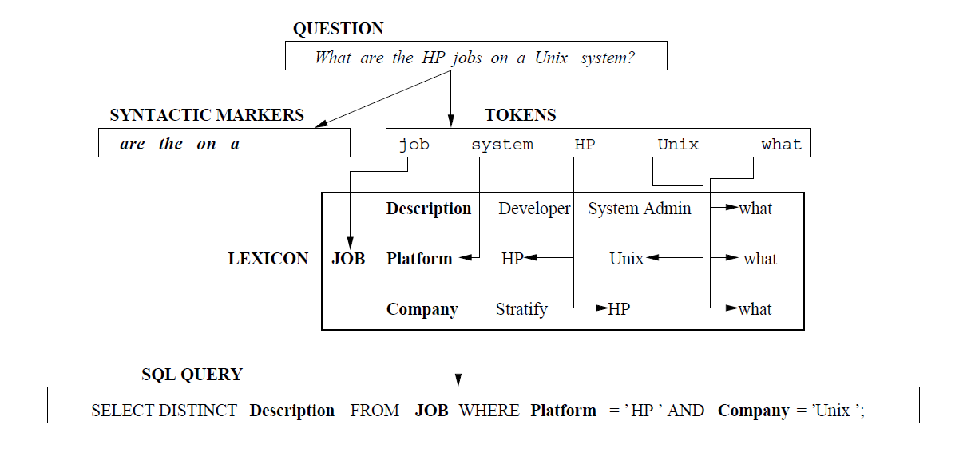
\includegraphics[scale=.7]{graficos/popescu-example}
  \caption{La traducción de la pregunta ``What are the HP jobs on a Unix system?'' a una consulta SQL}
  \label{fig:popescu-example}
\end{figure}

\end{frame}


\begin{frame}

\frametitle{Ejemplo}

\begin{figure}
  \centering
    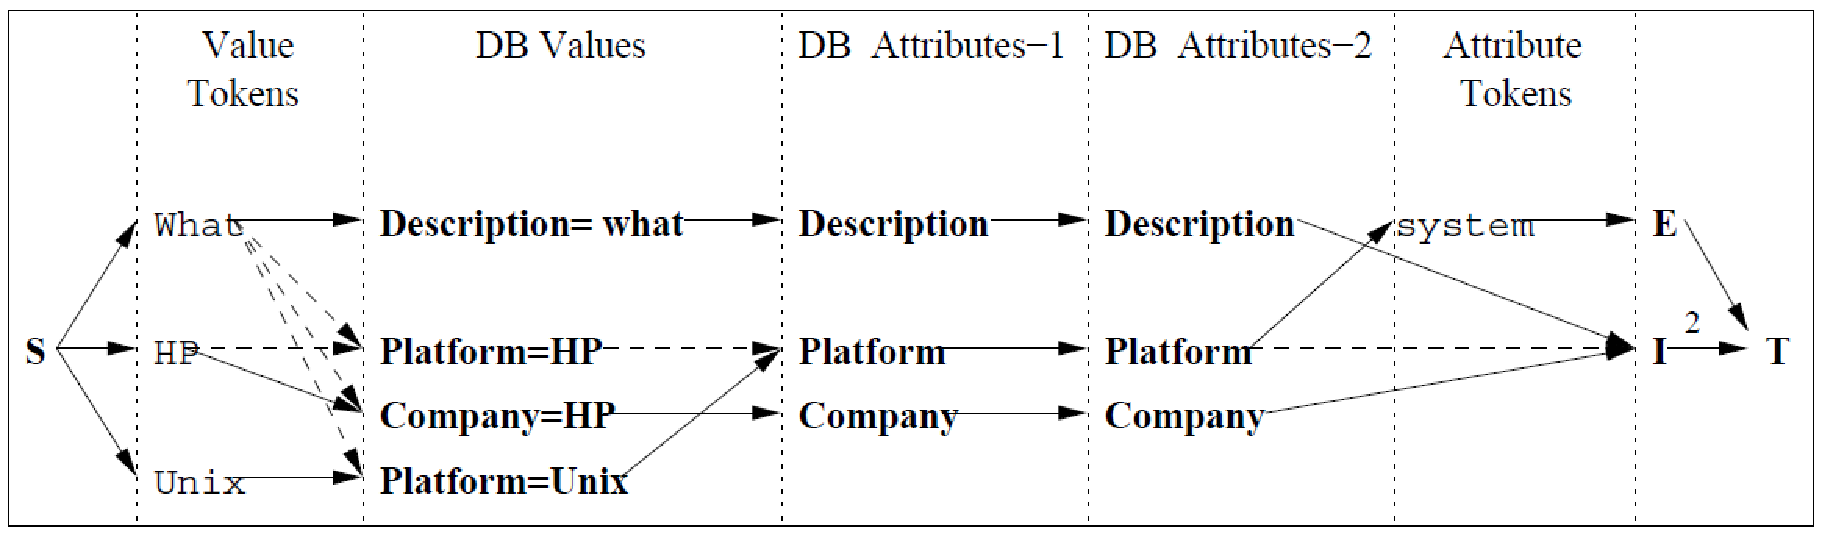
\includegraphics[scale=0.3]{graficos/popescu-example-2}
  \caption{El grafo de atributos y valores creado por Precise para la pregunta ``What are the HP jobs on a Unix system?''}
  \label{fig:popescu-example-2}
\end{figure}
\end{frame}

\subsection{Implementación}
\subsubsection*{Base de datos}
\begin{frame}
\frametitle{Base de datos: World (Country, City y CountryLanguage)}
\begin{figure}
    %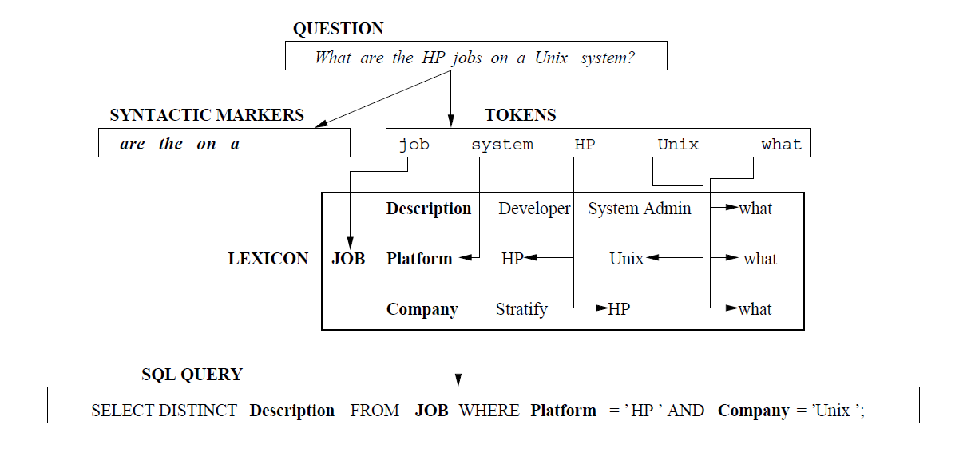
\includegraphics[scale=1.0]{graficos/popescu-example}
    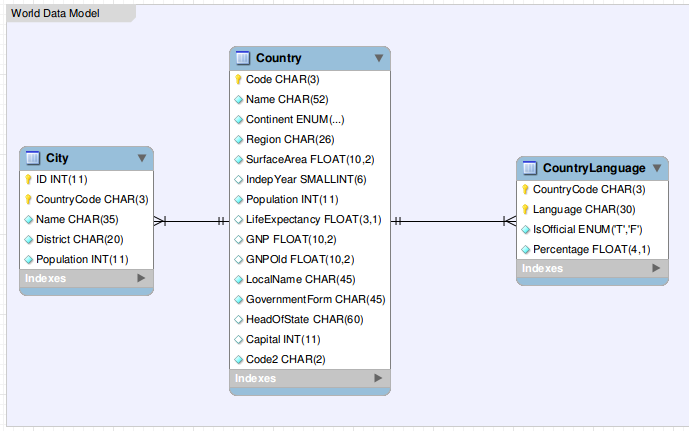
\includegraphics[width=9.823cm,height=6.004cm]{graficos/fuentes/world-db.png}
\end{figure}

\end{frame}
\subsubsection*{Implementación}
\begin{frame}
\frametitle{Lexicón}
  El lexicón es el módulo encargado de generar un conjunto de tokens para cada elemento de la base de datos. Una vez construido este conjunto, las responsabilidades del módulo son las siguientes:
\begin{itemize}
  \item Dado un lema, devolver el conjunto de tokens que lo contienen ($getTokens()$).
  \item Dado un token, devolver el conjunto de elementos de la base de datos que le \textit{corresponden} ($getMatchingElements()$).
  \item Wordnet. TokenAugmenter. Polisemia.
\end{itemize}
\end{frame}

\begin{frame}
\frametitle{TokenAugmenter}
\begin{center}
\begin{table}[h]
\centering
\begin{tabular}{| l |  p{8cm} |}
\hline
Elemento original & Sinónimos \\ \hline
head of state & president, leader, emperor, king \\ \hline
region & location\\ \hline
surface area & size, total size, square kilometers, km2\\ \hline
independence year & independent, independency\\ \hline
\end{tabular}
\caption{Sinónimos introducidos por el Token Augmenter}
\label{table:token-augmenter}
\end{table}
\end{center}
\end{frame}


\begin{frame}
\frametitle{Compatibilidad de Qwords}
\begin{center}
\begin{table}[h]
\centering
\begin{tabular}{| l |  p{8cm} |}
\hline
Qword & Atributos relacionados \\ \hline
What & \textbf{Name}, District, Population, Code, Continent, SurfaceArea, LifeExpectancy, GNP, LocalName, GovernmentForm,
                         Capital, IsOfficial, Percentage, Region \\ \hline
Which & Los mismos que para what\\ \hline
Where & \textbf{Region}, Continent, Capital, District\\ \hline
Who & \textbf{HeadOfState}\\ \hline
When & \textbf{IndependenceYear}\\ \hline
\end{tabular}
\caption{Atributos compatibles con cada Qword}
\label{table:atributos-qwords}
\end{table}
\end{center}

\end{frame}

\fontsize{9.5pt}{7.2}\selectfont
\begin{frame}
\frametitle{Tokenizer}
\begin{enumerate}
\item Separar la pregunta en palabras, eliminar puntuaciones y pasar a lower case.
\item Lematizar las palabras. Para esto usamos Freeling
\item Eliminar marcadores sintácticos.
\item Para cada lema, obtener todos los tokens que lo contienen del Lexicon (método getTokens).
\item Para cada token potencial (resultado del paso anterior) verificar que todos sus lemas estén presentes en el conjunto de lemas de la pregunta original.
\item Generar el conjunto de partes de todos los tokens hasta aquí obtenidos.
  Probando con cada elemento del conjunto de partes en lugar de utilizar solamente el conjunto original podemos obtener subconjuntos que cumplan también la condiciones requeridas para considerarse una tokenización completa (evaluados en 7).
\item Para cada uno de estos subconjuntos, verificar 1) que sus tokens cubran completamente los lemas significativos de la pregunta original y 2) que no haya lemas repetidos entre los tokens.
\end{enumerate}
\end{frame}

\begin{frame}
\frametitle{Matcher}
  
  \begin{itemize}
    \item Input = tokenizaciones completas generadas por el Tokenizer,
    \item Construye el grafo {\color{red} que expusimos en la sección NADA}
    \item Algoritmo de max flow. \footnotemark \footnotemark
    \item Las aristas implicadas en el flujo máximo posible asocian 
    \begin{itemize}
      \item 1) los tokens de valor y de atributo y los correspondientes elementos (valores y atributos, respectivamente) de la base de datos y 
      \item 2) pares de valores y atributos entre sí.
    \end{itemize}
    \item Otras soluciones posibles. Si el flujo es igual a la cantidad de tokens de valor en la pregunta es potencialmente una traducción válida. Retiramos ordenadamente las aristas del grafo que ocurren entre la columna 2 y 3 (tokens de valor y valores de la db).
\end{itemize}

\footnotetext[1]{\footnotesize{El problema de max-flow es un problema de grafos que consiste en “enviar” el máximo flujo posible a través de un grafo dirigido con dos nodos especiales (fuente o source y sumidero o sink) y aristas con cierta capacidad mayor o igual que cero. Este flujo debe ir desde el nodo fuente al nodo sumidero, respetando las capacidades de las aristas y respetando que, para cada nodo, el flujo saliente no puede ser mayor al flujo entrante. \url{http://web.mit.edu/~ecprice/acm/acm08/MaxFlow.java}}}

\footnotetext[2]{\footnotesize{Bloquee alguna funcionalidad basica por pajero.}}


%Cabe notarse aquí, como ya mencionamos anteriormente, que no soportamos en nuestra implementación la desambiguación de tokens de relación. Esto significa que: asumimos que un token de relación tiene un solo elemento relación asociado y no será necesario decidir si refiere a una relación u a otra. En todos los ejemplos de bases de datos que consideramos, esta asunción era verdadera (es decir, no existía un token de relación que necesite ser desambiguado) y por ello no implementamos esta capacidad del sistema, que quedará como trabajo futuro. Así mismo, no soportamos tokens multi tipados, prefiriendo relaciones sobre atributos y valores y atributos sobre valores (el caso implementativo es simple: require un grafo extra por cada combinación de tipos distintos por token). Los casos en que esta ambigüedad ocurría eran específicos y la solución no reportaba ninguna mejora cualitativa, por lo que lo dejamos de lado, quedando como una mejora futura.


\end{frame}

\begin{frame}
\frametitle{Matcher: condiciones}

Finalmente, verificamos cuales de las soluciones con máximo flujo cumplen las condiciones requeridas para ser una traducción válida según enunciamos en \ref{subsec:closed-domain}:

\begin{enumerate}
\item Todos  los tokens de la tokenización tienen un único elemento de la base de datos asociado y no hay elementos de la base de datos repetidos. (Mapping.meetsConditionOne())
\item Cada token de atributo se relaciona con un único token de valor respetando que: (Mapping.meetsConditionTwo())
\begin{enumerate}
\item el atributo relacionado con el token de atributo y el valor relacionado con el token de valor son compatibles (esta condición está garantizada por el max-flow mismo)
\item ambos tokens están sintácticamente asociados
\end{enumerate}
\item Cada token de relación está relacionado a un token de atributo o bien a un token de valor, cumpliendo las siguientes condiciones: (Mapping.meetsConditionThree())
\begin{enumerate}
\item la relación de la base de datos que corresponde al token de relación y el elemento de la base de datos que corresponde al token de atributo o token de valor son compatibles
\item ambos tokens (token de relación - token de atributo o bien token de relación - token de valor) están sintácticamente asociados
\end{enumerate}
\item La pregunta tiene una qword (Mapping.hasOneWhValue())
\end{enumerate}

Notemos que la condición 3 implica que para cada token de relación exista algún token de atributo o de valor a) compatible y b) sintácticamente asociado. La condición a) no está verificada por el algoritmo de máximo flujo y es verificada en el método Mapping.valid()

\end{frame}

\begin{frame}
\frametitle{Matcher: notas}
La definición de las reglas se hizo a prueba y error y es posible que sea simple, para alguien con mayores conocimientos lingüísticos, mejorarlas. Probablemente tenga sentido diferenciar entre sustantivos principal y modificador (Unix y system, por ejemplo) y modificar las reglas 3 y 4 para conectar solo los principales, entre otras mejoras. El sistema ofrece también la opción de no evaluar las asociaciones sintácticas en absoluto, en cuyo caso se mejora la performance pero aparecen nuevas traducciones válidas que podrían haber sido filtradas por estas condiciones, que el usuario deberá desambiguar manualmente).
Además, estas reglas seguramente sean insuficientes y estén dejando afuera varias preguntas que deberían poder procesarse.

Finalmente, todos los resultados de max-flow que cumplen con las condiciones de 1 a  4 son traducciones válidas, que pasan al MappingFilter, que realiza ciertos filtrados que describiremos, de nuevo, en un título aparte.

El resultado de este módulo es una lista de Mappings (una estructura que contiene 1) una tokenización completa de la pregunta original y 2) un mapeo válido entre cada token de la misma en un elemento de la base de datos). Cada mapeo es una traducción válida de la pregunta. Si existe solo uno, entonces este mapeo se traducirá en una query que generará el resultado. Si no, corresponde al MappingFilter realizar filtrados inteligentes de las múltiples soluciones y, en caso de que continuen existiendo múltiples soluciones, entonces se consultará al usuario qué quiso preguntar. Por otro lado, si no fue posible generar ninguna traducción válida, se retornará al usuario sin respuesta, pidiéndole que vuelva a escribir su pregunta de otro modo.


\end{frame}



\begin{frame}
\frametitle{Charniak}
Para verificar las condiciones de asociación sintáctica (2.b y 3.b) utilizamos la implementación oficial del árbol sintáctico de Charniak (\url{github.com/BLLIP/bllip-parser}), con un wrapper en java que es la clase $uba.nlp.CharniakParseTree$. Las reglas sintácticas utilizadas por Precise no están especificadas en los trabajos, por lo que creamos nuestras propias reglas tomando los ejemplos de asociaciones sintácticas dadas en los trabajos, evaluando los resultados de diferentes ejemplos y extrapolando reglas a partir de allí.


Veamos, en primer lugar, ejemplos del parse tree para tres preguntas:

\end{frame}

\begin{frame}
\frametitle{Charniak}
\Tree [.S1 [.WHNP [.WP What ] ] [.SQ [.VP [.AUX are ] [.NP [.DT the ] [.NNP HP ] [.NNS jobs ] ] [.PP [.IN on ] [.NP [.DT a ] [.NNP Unix ] [.NN system ] ] ] ] ] [.. ? ] ] \\
``What are the HP jobs on a Unix system?''

\end{frame}

\begin{frame}
\frametitle{Charniak}

\Tree [.S1 [.WHNP [.WP What ] ] [.SQ [.VP [.AUX are ] [.NP [.NP [.DT the ] [.NNS capitals ] ] [.PP [.IN of ] [.NP [.DT the ] [.NNP US ] [.NNS states ] ] ] ] ] ] [.. ? ] ] \\
``What are the capitals of the US states?''

\end{frame}


\begin{frame}
\frametitle{Charniak: reglas}
as reglas que construimos son las siguientes (notar que los nombres pueden denotar una direccionalidad, pero las relaciones son simétricas).
Utilizamos NNx para denotar cualquier hoja sustantivo, adjetivo o adverbio (JJ, JJR, JJS, NN, NNS, NNP, NNPS, RB, RBR, RBS, CD), NN para denotar estrictamente sustantivos (NN, NNS, NNP, NNPS), Nx para denotar cualquier sintagma relacionado a estos tipos de hojas (nodos intermedios): (ADJP, ADVP, NP, S) y Wx para denotar alguna de estas hojas: WDT, WP, WP\$ y WRB.

\begin{enumerate}
\item Hermanos:
  \begin{itemize}
    \item  NNx $\Leftrightarrow$ NNx $\Leftrightarrow$ Wx si comparten el mismo el mismo padre
  \end{itemize}
\item Qwords a sustantivo:
  \begin{itemize}
    \item Una Wx dentro de un WHNP $\Rightarrow$ un NN dentro de uno o más Nx dentro de un VP dentro de un SQ con el mismo SBARQ como padre que la WHNP mencionada.
  \end{itemize}
\item Sintagma nominal a sintagma preposicional:
  \begin{itemize}
    \item NN dentro de un Nx (1) $\Rightarrow$ NNx dentro de uno o más Nx dentro de un PP con el mismo padre que el Nx marcado con el (1)
  \end{itemize}
\item Sintagma nominal a sintagma verbal
    \begin{itemize}
      \item NN dentro de un Nx (1) $\Rightarrow$ NNx dentro de uno o más Nx dentro de un VP del mismo padre que el Nx marcado con el (1)
    \end{itemize}
\item Sintagma preposicional a sintagma preposicional:
  \begin{itemize}
    \item NNx dentro de un PP (1) $\Rightarrow$ NNx dentro de uno o más Nx dentro de un PP con el mismo padre que el PP marcado con el (1)
  \end{itemize}
  \item Términos a tokens:
  \begin{itemize}
    \item Dos tokens están asociados si cualquier término de uno está asociado a cualquier término de otro.
  \end{itemize}
\end{enumerate}


En los ejemplos presentados, los pares de términos asociados según estas reglas son los siguientes. Para el primero, (hp, jobs), (unix, system)  (regla 1), (what, hp), (what, jobs) (regla 2) y, finalmente, (hp, unix), (hp, system), (job, unix), (jobs, system) (regla 3). Para el segundo, (us, states) (regla 1), (what, capitals) (regla 2) y (capitals, us) y (capitals, states) (regla 3). Para el tercero, (what, names) (regla 2), (names, cities) y (cities, argentina) (regla 3).

\end{frame}


\begin{frame}
\frametitle{MappingFilter, QueryGenerator, MainProcessor}

\textbf{MappingFilter}

La clase $uba.app.MappingFilter$ es responsable, en primer lugar, de quitar las traducciones válidas repetidas y, en segundo lugar, de aplicar una serie de reglas también de filtrado. Para eliminar las traducciones repetidas, las transformamos en queries y simplemente comparamos por igualdad, ya que el generador de queries ordena las cláusulas generando, para inputs iguales pero diferentemente ordenados, la misma query.
Además de este filtro, aplicamos tres reglas más, de creación propia. En primer lugar, eliminamos ``semi duplicados'', que consisten en atributos similares en la base de datos, en concreto, para esta base de datos, consideramos semi-duplicada a una query que consulta por Country.Name y por Country.LocalName solamente. La segunda y la tercera regla están basadas en la siguiente idea: en el caso en que exista más de una traducción válida en la cual la qword esté asociada con un atributo \textit{implícito}, por como está el sistema definido, también estará asociado con todos los atributos que pueda estarlo (ver tabla table:atributos-qwords para las compatibilidades definidas). Esto implica que, por ejemplo, para cualquier pregunta cuya qword sea 'what' y no tenga su atributo asociado explícito, habrá 16 diferentes traducciones válidas. En los trabajos sobre los que basamos nuestro proyecto este problema no está mencionado y en los ejemplos presentados no es visible. Lo que hicimos en este caso es aplicar dos conceptos de preferencia. La segunda regla prefiere, entre los atributos implícitos posibles, aquellos cuya relación está mencionada en la pregunta (si hubiera alguna). La tercer regla señala un orden de preferencia entre los atributos mismos, una vez especificada la relación. El atributo implicito preferido está marcado en negrita en la tablatable:atributos-qwords. Si tras aplicar estar reglas siguen existiendo más de una traducción válida, entonces damos al usuario el control, pidiendo por una desambiguación.


\textbf{QueryGenerator}

El procedimiento para generar una query a partir de una traducción válida es exactamente el mismo que se desarrollo en subsec:closed-domain y está implementado en el método Mapping.query().


\textbf{MainProcessor}

Finalmente, el punto de entrada de todo el sistema es $uba.app.MainProcessor$, que puede utilizarse especificando el parámetro -q QUESTION en cuyo caso responderá a esa pregunta y retornará el control o bien sin parámetros, en cuyo caso ingresa en un loop de preguntas-respuestas. El resultado para cada pregunta es cero, una o más queries de SQL.
Agregamos la opción de desambiguación para que el usuario elija entre dos o más queries si no se pudo generar una y también una presentación de las respuestas una vez determinada la query final, pero es más bien experimental y poco sólido.
\end{frame}

\subsubsection*{Ejemplos}
\begin{frame}
\frametitle{Ejemplos}
  \begin{itemize}
    \item {\color{red} FILL ME}
    \item Who is the head of state of Zimbabwe?
    \item What caribbean countries are also considered north american?
  \end{itemize}
\end{frame}
\subsubsection*{Conclusiones y limitaciones}
\begin{frame}
\frametitle{Conclusiones y limitaciones}
  \begin{itemize}
    \item {\color{red} FILL ME}
  \end{itemize}
\end{frame}
